\documentclass[tikz]{standalone}

\usepackage{fontspec}
\setmainfont[Ligatures=TeX, Mapping=tex-text]{Lato}
\setmonofont{FreeMonoBold}
\usepackage{tikz}
\usetikzlibrary{arrows.meta}
\usepackage{xfp}

\begin{document}
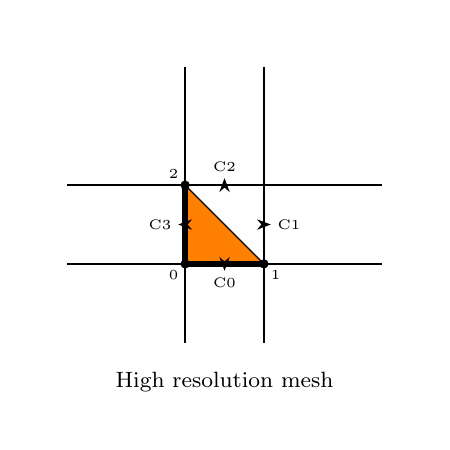
\begin{tikzpicture}

\def\width{5}
\def\height{5}
\def\ox{\fpeval{\width /2}}
\def\oy{\fpeval{\height /2}}

\tiny
\path [use as bounding box] (0,0) rectangle (\width,\height);

% SHAPE
\filldraw [line width=0.5pt, fill=orange] (\ox,\oy)
	+(-0.5,-0.5) node[draw, fill=black, circle, inner sep=1pt] {} node[below left] {0} --
	+(0.5,-0.5) node[draw, fill=black, circle, inner sep=1pt] {} node[below right] {1} --
	+(-0.5,0.5)  node[draw, fill=black, circle, inner sep=1pt] {} node[above left] {2}  --
	cycle;

% PORTS
\draw [line width=2pt] (\ox,\oy) ++(-0.5,0) +(0,-0.5) -- +(0,0.5);
\draw [line width=2pt] (\ox,\oy) ++(0,-0.5) +(-0.5,0) -- +(0.5,0);

% MESH
\draw [line width=0.5pt] (\ox,\oy) ++(0,-0.5) +(-2,0) -- +(2,0);
\draw [line width=0.5pt] (\ox,\oy) ++(0,0.5) +(-2,0) -- +(2,0);
\draw [line width=0.5pt] (\ox,\oy) ++(-0.5,0) +(0,-1.5) -- +(0,2);
\draw [line width=0.5pt] (\ox,\oy) ++(0.5,0) +(0,-1.5) -- +(0,2);
\path [tips, -{Stealth[length=5pt]}](\ox,\oy) ++(0,-0.5) -- +(0,-2.5pt) node[below] {C0};
\path [tips, -{Stealth[length=5pt]}](\ox,\oy) ++(0.5,0) -- +(2.5pt,0) node[right] {C1};
\path [tips, -{Stealth[length=5pt]}](\ox,\oy) ++(0,0.5) -- +(0,2.5pt) node[above] {C2};
\path [tips, -{Stealth[length=5pt]}](\ox,\oy) ++(-0.5,0) -- +(-2.5pt,0) node[left] {C3};

% NOTE
\draw (\ox,\oy) ++(0,-2) node {\footnotesize High resolution mesh};

\end{tikzpicture}
\end{document}
